\documentclass[twocolumn]{aastex61}
%\documentclass{emulateapj}
%\usepackage[colorlinks,urlcolor=blue,citecolor=blue,linkcolor=blue]{hyperref} 
\usepackage{graphicx,natbib}
\citestyle{aa}
\usepackage[space]{grffile}
\usepackage{latexsym}
\usepackage{amsfonts,amsmath,amssymb}
\usepackage{url}
\usepackage[utf8]{inputenc}
\usepackage{fancyref}
\usepackage{hyperref}
\usepackage{multirow}
\hypersetup{colorlinks=false,pdfborder={0 0 0},}

\newcommand{\rf}{\emph{realfast}}
\newcommand{\frb}{FRB 121102}

\begin{document}

\title{The \frb\ Campaign: Multi-Observatory Radio Burst and Implications for the FRB Population}
\shorttitle{\frb\ Observing Campaign}
\shortauthors{Law et al.}

\author[0000-0002-4119-9963]{C.~J.~Law}
\affiliation{Department of Astronomy and Radio Astronomy Lab, University of California, Berkeley, CA 94720, USA}

\author{C.~G.~Bassa}
\affiliation{ASTRON, Netherlands Institute for Radio Astronomy, Postbus 2, 7990 AA, Dwingeloo, The Netherlands}

\author{G.~C.~Bower}
\affiliation{Academia Sinica Institute of Astronomy and Astrophysics, 645 N. A'ohoku Place, Hilo, HI 96720, USA}

\author{S.~Burke-Spolaor}
\affiliation{National Radio Astronomy Observatory, Socorro, NM 87801, USA}
\affiliation{Department of Physics and Astronomy, West Virginia University, Morgantown, WV 26506, USA}
\affiliation{Center for Gravitational Waves and Cosmology, West Virginia University, Chestnut Ridge Research Building, Morgantown, WV 26505}

\author{B.~J.~Butler}
\affiliation{National Radio Astronomy Observatory, Socorro, NM 87801, USA}

\author{T.~Cantwell}
\affiliation{Jodrell Bank Centre for Astrophysics, Alan Turning Building, School of Physics \& Astronomy ,The University of Manchester, Oxford Road, Manchester M13 9PL, UK}

\author{S.~H.~Carey}
\affiliation{Astrophysics Group, Cavendish Laboratory, 19 J. J. Thomson Avenue, Cambridge CB3 0HE, UK}

\author{S.~Chatterjee}
\affiliation{Cornell Center for Astrophysics and Planetary Science and Department of Astronomy, Cornell University, Ithaca, NY 14853, USA}

\author{J.~M.~Cordes}
\affiliation{Cornell Center for Astrophysics and Planetary Science and Department of Astronomy, Cornell University, Ithaca, NY 14853, USA}

\author{P.~Demorest}
\affiliation{National Radio Astronomy Observatory, Socorro, NM 87801, USA}

\author{R.~Fender}
\affiliation{Centre for Astrophysical Surveys, University of Oxford, Denys Wilkinson Building, Keble Road, Oxford OX1 3RH, UK}

\author{K.~Grainge}
\affiliation{Jodrell Bank Centre for Astrophysics, Alan Turning Building, School of Physics \& Astronomy ,The University of Manchester, Oxford Road, Manchester M13 9PL, UK}

\author{J.~W.~T.~Hessels}
\affiliation{ASTRON, Netherlands Institute for Radio Astronomy, Postbus 2, 7990 AA, Dwingeloo, The Netherlands}
\affiliation{Anton Pannekoek Institute for Astronomy, University of Amsterdam, Science Park 904, 1098 XH Amsterdam, The Netherlands}

\author{J.~Hickish}
\affiliation{Dept of Astronomy and Radio Astronomy Lab, University of California, Berkeley, CA 94720, USA}
\affiliation{Astrophysics Group, Cavendish Laboratory, 19 J. J. Thomson Avenue, Cambridge CB3 0HE, UK}

\author{V.~M.~Kaspi}
\affiliation{Department of Physics and McGill Space Institute, McGill University, 3600 University St., Montreal, QC H3A 2T8, Canada}

\author{T.~J.~W.~Lazio}
\affiliation{Jet Propulsion Laboratory, California Institute of Technology, Pasadena, CA 91109, USA}

\author{M.~A.~McLaughlin}
\affiliation{Department of Physics and Astronomy, West Virginia University, Morgantown, WV 26506, USA}
\affiliation{Center for Gravitational Waves and Cosmology, West Virginia University, Chestnut Ridge Research Building, Morgantown, WV 26505}

\author{D.~Michilli}
\affiliation{ASTRON, Netherlands Institute for Radio Astronomy, Postbus 2, 7990 AA, Dwingeloo, The Netherlands}
\affiliation{Anton Pannekoek Institute for Astronomy, University of Amsterdam, Science Park 904, 1098 XH Amsterdam, The Netherlands}

\author{K.~Mooley}
\affiliation{Centre for Astrophysical Surveys, University of Oxford, Denys Wilkinson Building, Keble Road, Oxford OX1 3RH, UK}

\author{Y.~C.~Perrott}
\affiliation{Astrophysics Group, Cavendish Laboratory, 19 J. J. Thomson Avenue, Cambridge CB3 0HE, UK}

\author{S.~M.~Ransom}
\affiliation{National Radio Astronomy Observatory, Charlottesville, VA 22903, USA}

\author{N.~Razavi-Ghods}
\affiliation{Astrophysics Group, Cavendish Laboratory, 19 J. J. Thomson Avenue, Cambridge CB3 0HE, UK}

\author{M.~Rupen}
\affiliation{National Research Council of Canada, Herzberg Astronomy and Astrophysics, Dominion Radio Astrophysical Observatory, P.O. Box 248, Penticton, BC V2A 6J9, Canada}

\author{A.~Scaife}
\affiliation{Jodrell Bank Centre for Astrophysics, Alan Turning Building, School of Physics \& Astronomy ,The University of Manchester, Oxford Road, Manchester M13 9PL, UK}

\author{P.~Scott}
\affiliation{University of Cambridge, UK}

\author{P.~Scholz}
\affiliation{National Research Council of Canada, Herzberg Astronomy and Astrophysics, Dominion Radio Astrophysical Observatory, P.O. Box 248, Penticton, BC V2A 6J9, Canada}

\author{A.~Seymour}
\affiliation{Arecibo Observatory, HC3 Box 53995, Arecibo, PR 00612, USA}
\affiliation{Max-Planck-Institut f\"ur Radioastronomie, Auf dem H\"ugel 69, Bonn, D-53121, Germany}

\author{L.~G.~Spitler}
\affiliation{Max-Planck-Institut f\"ur Radioastronomie, Auf dem H\"ugel 69, D-53121 Bonn, Germany}

\author{S.~P.~Tendulkar}
\affiliation{Department of Physics and McGill Space Institute, McGill University, 3600 University St., Montreal, QC H3A 2T8, Canada}

\author{D.~Titterington}
\affiliation{University of Cambridge, UK}

\author{R.~S.~Wharton}
\affiliation{Cornell Center for Astrophysics and Planetary Science and Department of Astronomy, Cornell University, Ithaca, NY 14853, USA}

\author{P.~K.~G.~Williams}
\affiliation{Harvard-Smithsonian Center for Astrophysics, Cambridge, MA, USA}

\begin{abstract}
The recent precision localization of \frb\ has helped identify its host galaxy, measure its distance, and establish it as a member of a truly new class of astrophysical source. We present results of the coordinated observing campaign that made this localization, including the first simultaneous detection of an FRB burst with multiple telescopes. Of the nine bursts detected by the Very Large Array at 3~GHz, four had simultaneous observing coverage at other observatories, and one was detected by the Arecibo Observatory at 1.4~GHz. We show that the burst spectra typically have a broad shape that tapers off on scales of $\sim500$~MHz, plus fine spectral structure on MHz-frequency scales. We present the first FRB energy distribution and temporal statistics for \frb\ and argue that the whole FRB population is adequately described by a single class similar to \frb. 
*population models* *slsn*
**This source shows that optimal FRB survey strategies should...**
\end{abstract}

\section{Introduction}

Fast Radio Bursts (FRBs) were discovered ten years ago as a millisecond-duration radio transient with an anomalously high dispersion measure \citep[the ``Lorimer burst'';][]{2007Sci...318..777L}. Their large dispersion measure (DM) implied that they originated outside of our Galaxy, potentially at cosmological distances, and were orders of magnitude more luminous than any other millisecond radio transient \citep{2013Sci...341...53T}. Both their energetics and distance have inspired a wide variety of models and astrophysical applications \citep[e.g.,][]{2014ApJ...780L..33M, 2014ApJ...797...70K, 2016MNRAS.458L..19C, 2016MNRAS.457..232C}. However, that potential was limited by the lack of a definitive association of an FRB to an extragalactic host.

This paper is part of a series based on the first localization of an FRB and its unambiguous association to an extragalactic host \citep{LOC, OPT, EVN}. \frb, also known as the ``repeating FRB'', was first detected in November 2012 by the Arecibo Observatory \citep{2014ApJ...790..101S}. In mid 2015, new Arecibo observations revealed a series of bursts at the same DM ($\sim559$\ pc cm$^{-3}$) and sky position demonstrating that it repeats \citep{2016Natur.531..202S}. Beginning in August of 2015, we made the first of nine detections of \frb\ with the Very Large Array \citep{LOC} and localized it with a precision of 0.1\arcsec. Subsequent radio and optical observing discovered more bursts from \frb\ and associated them with a persistent radio and optical source at a redshift of 0.193 with a precision of 0.01" \citep[$\sim40$\ pc]{OPT, EVN}.

\frb\ has now been localized four orders of magnitude better than any other FRB and placed at a cosmological distance. Its lookback and luminosity distances are 746 and 972 Mpc, assuming a concordance cosmology with parameters given by \citet{2016A&A...594A..13P}. This association means that \frb\ is orders of magnitude more luminous than any other millisecond transient and that its DM traces both the host and intergalactic medium \citep{OPT}. If \frb\ is representative of all FRBs, then we should expect them to be useful as probes of the intergalactic medium and their host galaxies. Thus, the confirmation of a cosmological distance for \frb\ has begun to fulfil the promise implied by the Lorimer burst.

Although new models of FRB origin have been already been developed \citep{2017arXiv170104815K, 2017arXiv170102370M, 2017arXiv170104094Z, 2017arXiv170102492D}, we still do not know what causes them. 
**magnetar birth?**
Also, it has not been demonstrated that \frb\ is representative of the overall FRB population. In fact, the repetition of its bursts is unique among all FRBs \citep{2015MNRAS.454..457P}, so it is natural to ask whether \frb\ is representative. An important first step is to demonstrate that the properties of \frb\ are consistent with the significant body of facts for the overall population \citep{2015MNRAS.451.3278M, 2016MPLA...3130013K}. The repeating nature of \frb\ provides us with a sample of bursts covering a range of spectral properties, temporal properties, and luminosities that can be used to test its connection to the larger FRB population.

We can also assume that \frb\ is representative of all FRBs and use it to constrain the physical processes at play in the overall FRB population. In this case, we know that FRBs are apparently luminous, but if that is due to intrinsic processes, such as coherent, pulsar-like emission \citep{2014PhRvD..89j3009K, 2014ApJ...785L..26L, 2016MNRAS.457..232C}, or extrinsic effects like scintillation \citep{CORDES}. The paper presents an analysis of the spectral properties of VLA bursts implied by simultaneous observing at Effelsberg, GBT, AMI-LA, and Arecibo, including the first simultaneous detection of an FRB at two observatories. The repetition of \frb\ also has strong implications for calculations of their rate of occurrence \citep{2016MNRAS.458L..89C} and comparison to other classes of transient, such as superluminous supernovae \citep{OPT}.

This paper opens by describing the multi-telescope observing campaign and a refined analysis of the nine VLA bursts. Next, we present the spectrum of a burst from \frb\ that was simultaneously detected by the VLA and Arecibo observatories. **Simulations of temporal statistics and luminosity distribution...** **New estimate of FRB rate and comparison to other transient populations** We close with a discussion of how the \frb\ burst spectra, host properties, burst rate estimates, and other properties inform new strategies for finding FRBs.

\section{Observations}

\begin{figure*}[t]
\begin{center}
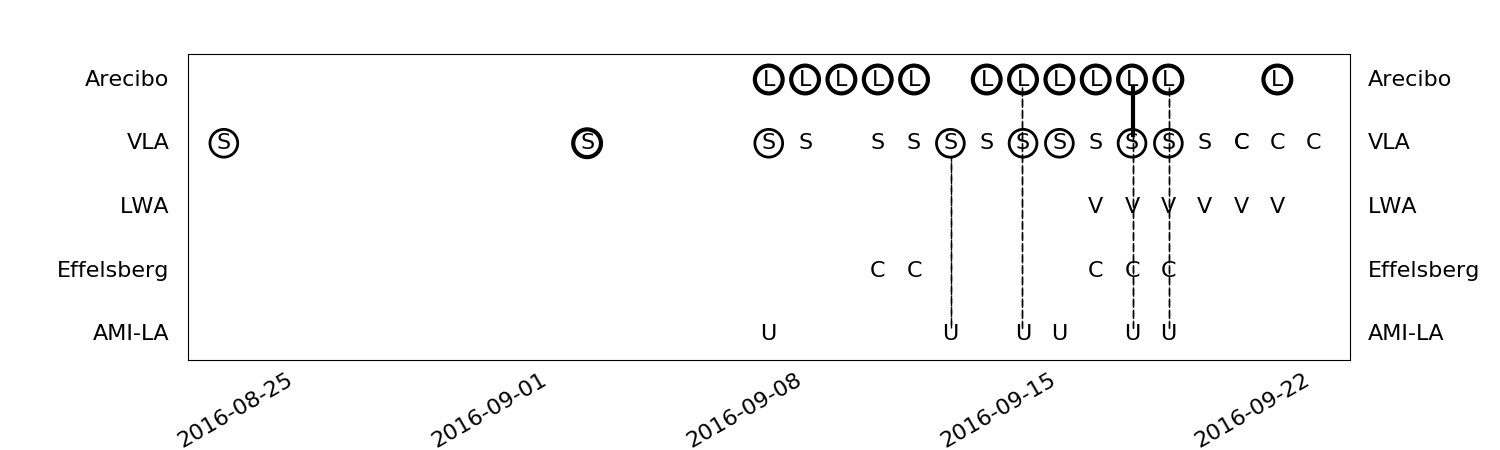
\includegraphics[width=2\columnwidth]{timeline}
\caption{Summary of late-2016 observing coverage and detections of \frb\ during the multi-telescope observing campaign. Symbols show days with observations and circles highlight observations that detected bursts from \frb. Multiple circles indicate multiple burst detections, except for Arecibo, which typically has multiple detections per observing session (a detailed analysis is left for a future paper). The black dashed lines show the VLA burst detections with simultaneous coverage at other telescopes. The solid black line shows the simultaneous burst detection at VLA and Arecibo.
\label{fig:multi}}
\end{center}
\end{figure*}

The data presented here were obtained from multiple programs and telescopes, but focuses on an observing campaign in August/September 2016. The central goal was to interferometrically localize \frb\ with the VLA in coordination with Arecibo Observatory, with others included on a best-effort basis. We coordinated observing between the VLA, Arecibo, Effelsberg, and AMI-LA telescopes, as shown in Figure \ref{fig:multi}. Below, we summarize these observations, with a focus on those conducted simultaneously with VLA burst detections from \frb.

\subsection{VLA}
The \frb\ observing campaign started in late 2015 with a 10~hr campaign observed at 1.4~GHz in the compact D configuration. In April through May 2016, we conducted a 40~hr campaign at 3~GHz in the C and CnB configurations in coordination with Arecibo. We concluded with a 40~hr, coordinated campaign from August through September 2016 in the B configuration and during the move to the most extended A configuration. In the late-2016 campaign, the first 34 hours of VLA observations were made at 3~GHz, while the last 6 hours were observed at 6~GHz. This paper focuses on the data collected at 3~GHz, which includes all nine burst detections and is the widest bandwidth to have ever detected an FRB.

All VLA fast-sampled data were observed with 5~ms sampling, 256 channels, and dual-circular polarization \citep{2015ApJ...807...16L}. The channel frequency width was set to maximize sensitivity to the known DM of \frb with the largest total bandwidth. The total bandwidth at L (1.4~GHz), S (3~GHz), and C (6~GHz) bands was 256~MHz, 1024~MHz, and 2048~MHz, respectively. The 3~GHz data were recorded data in eight spectral windows with 32 channels each.

Observations in August and September were searched by a prototype version of \rf\footnote{See \url{http://realfast.io}.}. \rf\ is a real-time, fast imaging transient search system. The current prototype runs on CPU-based hardware that is normally dedicated to the VLA correlator; for this experiment, it runs the transient search pipeline software called \emph{rtpipe} \citep[\url{https://github.com/caseyjlaw/rtpipe};][]{2015ApJ...807...16L}. Images were formed for each integration with a DM grid of 0, 546, 556.9, 560, and 565 pc cm$^{-3}$ and a time resampling grid of 5, 10, 20, 40, and 80 ms. This DM grid was chosen to maintain 90\% sensitivity to the nominal DM range of 540--570 pc cm$^{-3}$, which includes the known \frb\ DM of 559 pc cm$^{-3}$. Gain calibration was made from observations of J0555+3948 by the ``telcal'' system, which uses phase-only calibration. A flux scale is calculated for each spectral window from an observation on {\color{red}xx (Bryan)} and applied to all burst spectra.

Burst detections and localizations were made within hours of data being recorded. The transient search starts when data are recorded and proceeds slower than real-time, so we refer to it as ``quasi real-time''. For each trial DM, integration, and time scale, we form an image and calculate the S/N ratio for the peak pixel in the dirty image. We empirically identified S/N thresholds of 6.4 and 7.4 as useful to capture data quality statistics and candidates for inspection, respectively. The higher threshold is relatively unlikely to be triggered by thermal noise in this configuration, so \rf\ generates a more detailed (and computationally intensive) candidate visualization that includes an image and spectrum. All visibilities are recorded so detailed analysis, including improved calibration and localization, can be conducted offline. 

Computational notebooks to reproduce the transient detection, localization, and analysis presented here can be found at \url{https://github.com/caseyjlaw/FRB121102}. Time cut-out visibility data and calibration products are available at \url{https://doi.org/10.7910/DVN/TLDKXG}. Original visibility data are available under VLA program codes 16A-459 and 16A-496 and can be downloaded at \url{http://archive.nrao.edu}.

\subsection{Arecibo}

During the late-2016 campaign, Arecibo observed with the L-wide receiver using the PUPPI pulsar backend. The observational frequency range was 1.15 to 1.73~GHz and frequency resolution was 1.5625~MHz. We recorded total full Stokes polarization intensity spectra with time at a resolution of 10.24~$\mu$s. Each frequency channel was coherently dedispersed to 557 pc cm$^{-3}$, thereby eliminating intra-channel dispersion smearing. The full width at half maximum (FWHM) beam size at band center is 3.3\arcmin.

In total, twelve Arecibo observations had some simultaneous coverage with the VLA. Four of those observations were simultaneous with bursts detected with the VLA and one of those observations detected the same VLA burst. During the first VLA burst with Arecibo coverage (MJD 57643), the PUPPI system failed so data were recorded with {\color{red} xx (Jason?)} at C band. No detection was made in those Arecibo data. Overall, there were many more bursts detected at Arecibo than with the VLA and a more detailed analysis of those bursts will be presented in a future paper.

\subsection{Effelsberg}

Effelsberg observations were conducted with the S60mm receiver at an observing frequency of 4.6 to 5.1~GHz. Total intensity spectra were recorded by the PFFTS backend in pulsar search mode with a time resolution of 65.5~$\mu$s and 128 frequency channels. The system equivalent flux density is 18 Jy and a FWHM beam size of 2.4\arcmin at 4.85~GHz. 

Five Effelsberg observations had some simultaneous coverage with the VLA, of which two were simultaneous with VLA bursts. Unfortunately, due to a configuration error, a 100~MHz bandwidth filter centered at 4.85~GHz was in place for both of these sessions. The sensitivity was about two times worse than the nominal value. No burst was detected in either observation.

\subsection{AMI-LA}

We observed \frb\ with the Arcminute MicroKelvin Imager Large Array (AMI-LA; Zwart et al. 2008) for 3 hours each on four epochs starting at MJDs 57643, 57645, 57648, and 57649. Observations were made with the new digital correlator having 4096 channels across a 5~GHz bandwidth between 13--18~GHz with a 1~s integration time. The phase calibrator, J0518+3306, was observed every 12 minutes for about 1.5 minutes. The AMI-LA data were binned to eight 0.625~GHz channels and processed (RFI excision and calibration) with a fully-automated pipeline, AMI-REDUCE \citep[e.g.,][]{2013MNRAS.429.3330P}. Daily measurements of 3C48 and 3C286 were used for the absolute flux calibration, which is good to about 10\%. 

We inspected the calibrated visibilities, and did not find any signal above 30 mJy in the 1s samples at and in the vicinity of the detected bursts. Concatenating and imaging the 12 hours of calibrated data with the CASA tasks {\it concat} and {\it clean} also does not yield any significant detection at the FRB location. Although the statistical $3\sigma$\ upper limit is 60 $\mu$Jy, extended mJy-level sources in the field cause sidelobe confusion (the AMI-LA angular resolution is $\sim$30\arcsec), and the actual upper limit is larger. We introduced artificial point sources at the FRB location using the CASA {\it sm} tool, and found that these sources can be recovered as long as their peak flux densities are more than $\sim100\mu$Jy. Hence, we place an upper limit of $100\pm10 \mu$Jy on any quiescent or possible radio flaring on $\sim$days timescales from the FRB. This limit is similar to the flux density measured by the VLA \citep{LOC}.

\section{Results}

\subsection{Multi-Observatory Burst Spectrum}
Four of the VLA bursts were observed simultaneously with Arecibo and AMI-LA (Figure \ref{fig:multi}). Of these, the burst on 57648 was detected by Arecibo at the same time (after correcting for the known DM of \frb). The Arecibo detection of this burst had a significance of {\color{red} xx$\sigma$ (Jason)}.

Figure {\color{red} **to do**} shows the dynamic spectrum formed from the phased VLA and Arecibo data... **Discuss dispersion correction, time alignment, chance of false association** 

This simultaneous detection of a burst from roughly 1.2 to 3.5~GHz shows that some bursts emit over more than an octave of frequency. However, the other three...**
**
 is one of three VLA bursts with L-band coverage by Arecibo, which implies that those bursts had a smaller spectral width. However, all three VLA bursts with L-band Arecibo observations were relatively weak, so it is difficult to rule out L-band emission entirely. However, as described in \S \ref{sec:spec}, some of the VLA bursts peak within the band from 2.5 to 3.5~GHz, which implies a much smaller spectral coverage for typical bursts.

\subsection{VLA Bursts}

\begin{figure*}[htb]
\begin{center}
% \begin{minipage}{2\columnwidth}
%  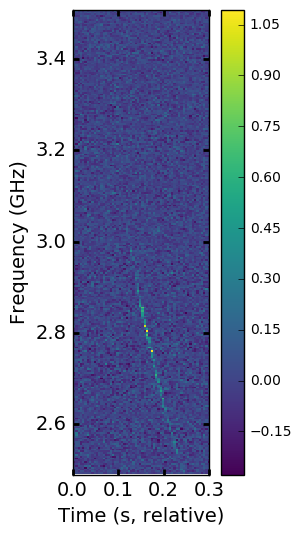
\includegraphics[width=0.18\columnwidth]{sgram_57623.png}
%  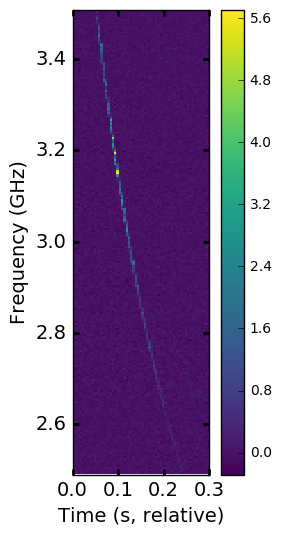
\includegraphics[width=0.18\columnwidth]{sgram_57633_scan7.png}
%  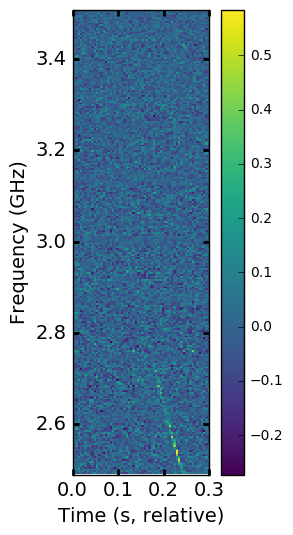
\includegraphics[width=0.18\columnwidth]{sgram_57633_scan13.png}
%  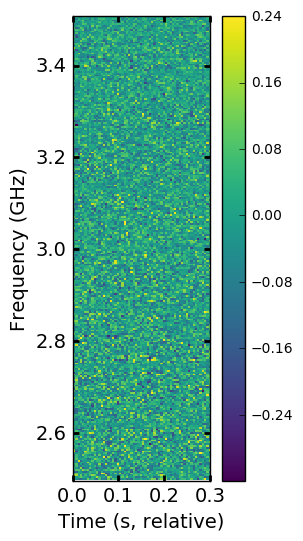
\includegraphics[width=0.18\columnwidth]{sgram_57638.png}
%  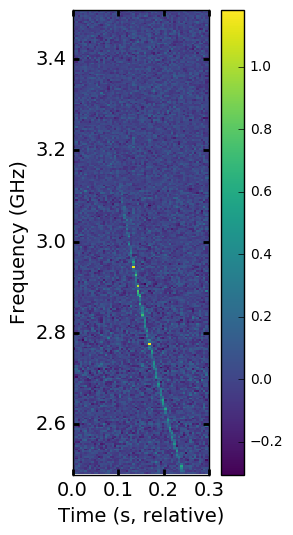
\includegraphics[width=0.18\columnwidth]{sgram_57643.png}
% \end{minipage}
%
% \begin{minipage}{2\columnwidth}
%  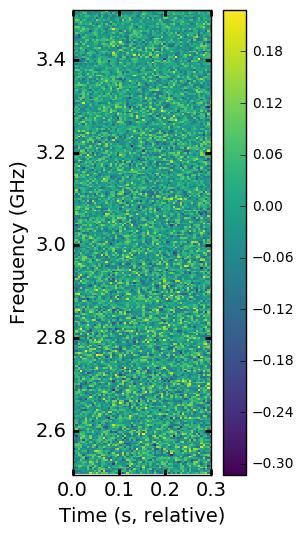
\includegraphics[width=0.18\columnwidth]{sgram_57645.png}
%  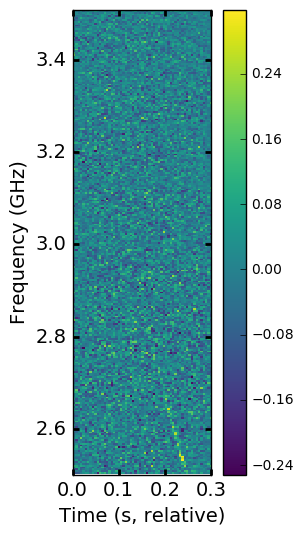
\includegraphics[width=0.18\columnwidth]{sgram_57646.png}
%  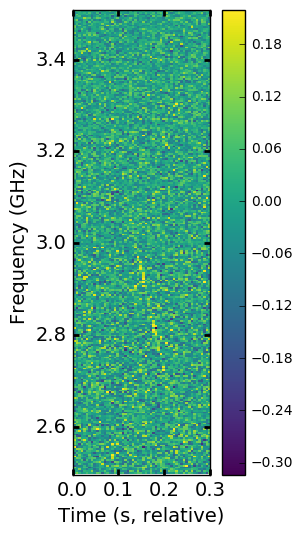
\includegraphics[width=0.18\columnwidth]{sgram_57648.png}
%  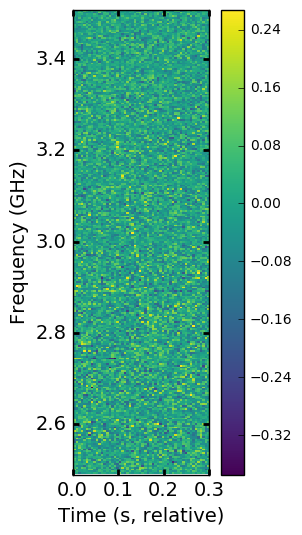
\includegraphics[width=0.18\columnwidth]{sgram_57649.png}
% \end{minipage}
%
% \caption{Dynamic spectra (time vs frequency intensity maps) for the nine VLA bursts. Starting at the top left, they correspond to bursts 57623, 57633.68, 57633.70, 57638, 57643, (bottom left) 57645, 57646, 57648, and 57649. Note that bursts are detected in 5~ms images generated from dedispersed visibilities.
 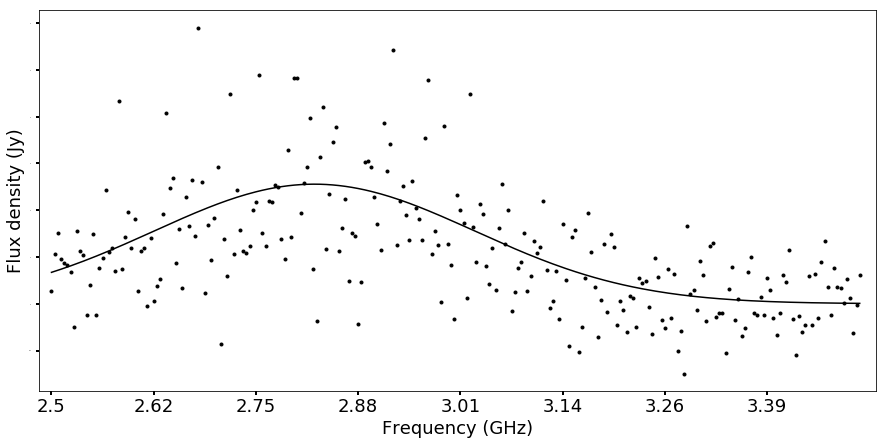
\includegraphics[width=1.9\columnwidth]{spec_57648.png}
 \caption{**Placeholder** Fill in with AO+VLA dynamic spectrum.
 \label{fig:sgram}}
\end{center}
\end{figure*}


\subsubsection{Spectral Modeling}
\label{sec:spec}
We used two techniques to refine the analysis of the nine VLA radio burst spectra described in \citet{LOC}. First, we improved on the initial analysis by using a better calibration scheme and optimizing the detection significance over a fine grid of DM ($\Delta \rm{DM}=1\ \rm{pc}\ \rm{cm}^{-3}$). After calibration and flagging, the visibility phases were rotated to the best-fit location \citep[(RA, Dec) $=$ (05h31m58.70s, +33d08m52.5s);][]{LOC} to extract a Stokes I spectrum that maximizes the image S/N for each burst. Table \ref{tab:spec} gives the resulting integrated burst flux density, image S/N, and Stokes V, while Figure \ref{fig:spec} shows the Stokes I spectra. Generally, the burst spectra are characterized by a broad, Gaussian shape with inter-channel modulation as high as 100\%.

\begin{table*}
\caption{Properties of Bursts from \frb}
\centering
\begin{tabular}{lcccccccc}
\hline
Date                & S$_{\rm{I,int}}$  & Image S/N & E$_{\rm{int}}$ & DM$_{\rm{opt}}$ & S$_{\rm{I,peak}}$ & Center & FWHM & S$_{\rm{V}}$ \\
(MJD)               & (mJy)           &           & ($10^{38}$\ erg) & (pc cm$^{-3})$ & (mJy) & (GHz)  & (MHz) & (mJy) \\ \hline
57623.74402686      & 194             & 38        & 11 & 562.1 & 690 & 2.8 & 290 & +3 \\ % 7.8  & 562.5 & 460 & 2.8 & 300 & +3 \\
57633.67986367      & 1500            & 179       & 97 & 561.3 & 3350 & 3.2 & 510 & --35 \\ % 65   & 561.4 & 2200 & 3.2 & 520 & --35 \\
57633.69515938\tablenotemark{a} & 69  & 15        & 7 & 555.8 & $>$430 & $<$2.5 & 290 & +2 \\ % 5.9  & 555.4 & $>$320 & $<$2.5 & $>$320 & +2 \\
57638.49937435      & 55              & 12        & 3 & 558.6 & 130 & 3.1 & 410 & +5 \\ % 1.8  & 554.9 & 70 & 3.1 & 440 & +5 \\
57643.45730263      & 508             & 100       & 34 & 558.7 & 1170 & 2.8 & 510 & --5 \\ % 13   & 559.3 & 440 & 2.8 & 530 & --5 \\
57645.42958602      & 64              & 13        & 4 & 555.9 & 170 & 2.8 & 380 & +3 \\ % 2.6  & 554.1 & 50 & 2.7 & 970 & +3 \\
57646.46600650\tablenotemark{a} & 87  & 20        & 10 & 562.4 & $>$420 & $<$2.5 & 420 & +1 \\ % 3.9  & 568.1 & $>$190 & $<$2.5 & $>$360 & +1 \\
57648.43691490\tablenotemark{b} & 111 & 25        & 7 & 557.4 & 260 & 2.8 & 470 & +9 \\ % 2.9  & 557.8 & 110 & 2.8 & 440 & +9 \\
57649.45175697      & 167             & 36        & 12 & 559.9 & 290 & 3.0 & 690 & +1 \\ \hline % 6.3  & 559.9 & 80 & 2.9 & 1400 & +1 \\ \hline
\end{tabular}
\tablenotetext{a}{Best-fit Gaussian is not centered in 3~GHz band, so spectral parameters are limits.}
\tablenotetext{b}{Detected simultaneously with Arecibo between 1.15 and 1.73~GHz.}
\label{tab:spec}
\end{table*} 

To better understand the spectra, we extracted dynamic radio spectra (time versus frequency) for 2d modeling with the MCMC sampler \emph{emcee} \citep{2013PASP..125..306F}. These dynamic spectral were modeled as the product of a Gaussian shape (amplitude, center, width) and a temporal shape (start time, DM, and width). These 6-dimensional fits were sampled with 100 walkers taking 500 steps; typically, the first 200 steps were used to burn in the walkers and were ignored. A flat prior was used over all ranges with valid data, including a requirement that the Gaussian integral produce a detection significance higher than 8$\sigma$. To represent the strong inter-channel modulation, the model error was estimated as the maximum of the modeled flux and the measured, off-burst noise value (typically 70 mJy per 5~ms integration and 4~MHz channel).

The parameters for the best model of the dynamic spectrum are given in Table \ref{tab:spec} and the resulting Gaussian model overlaid on Figure \ref{fig:spec}. The typical burst has a spectral width of 500~MHz. All but two of the best-fit Gaussians are centered inside the 3~GHz band and some appear contained by the 1~GHz wide band. This is consistent with previous detections of \frb\ by Arecibo, which showed quasi-broadband structure \citep{2016arXiv160308880S} and large variation in the implied spectral index \citep{2014ApJ...790..101S}. A detailed discussion of high-resolution \frb\ burst spectra seen by the Arecibo Observatory will be presented elsewhere \citep{WEIRD}.

\begin{figure*}[ht]
\begin{center}
 \begin{minipage}{2\columnwidth}
  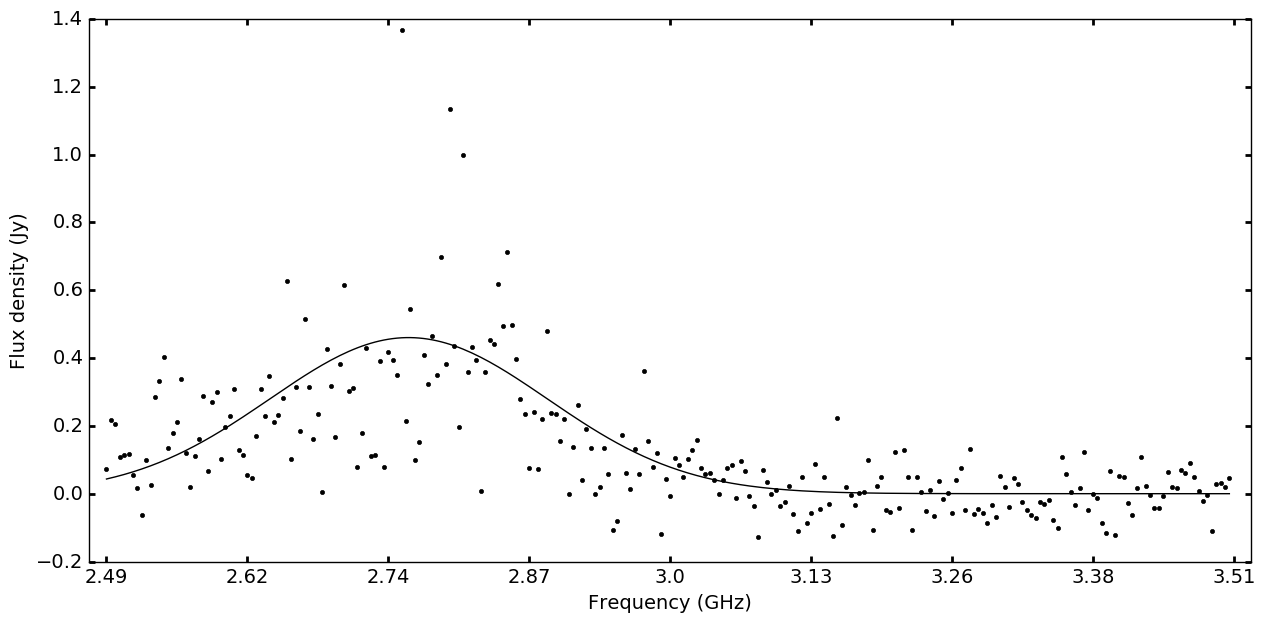
\includegraphics[width=0.33\columnwidth]{spec_57623.png}
  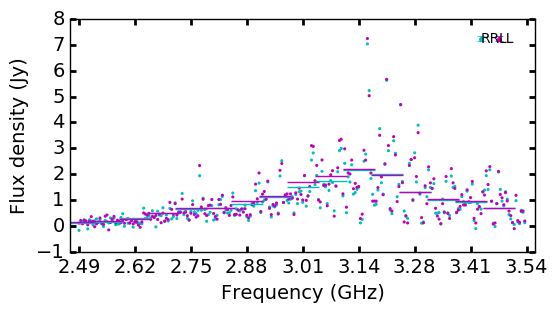
\includegraphics[width=0.33\columnwidth]{spec_57633_scan7.png}
  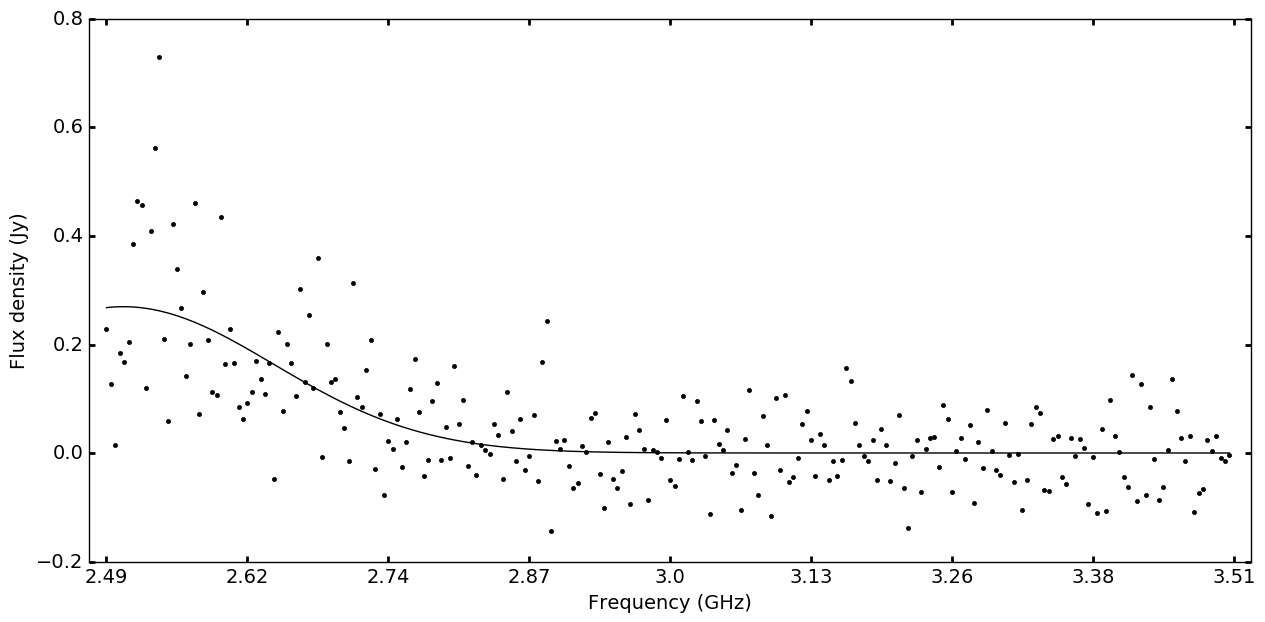
\includegraphics[width=0.33\columnwidth]{spec_57633_scan13.png}
 \end{minipage}

 \begin{minipage}{2\columnwidth}
  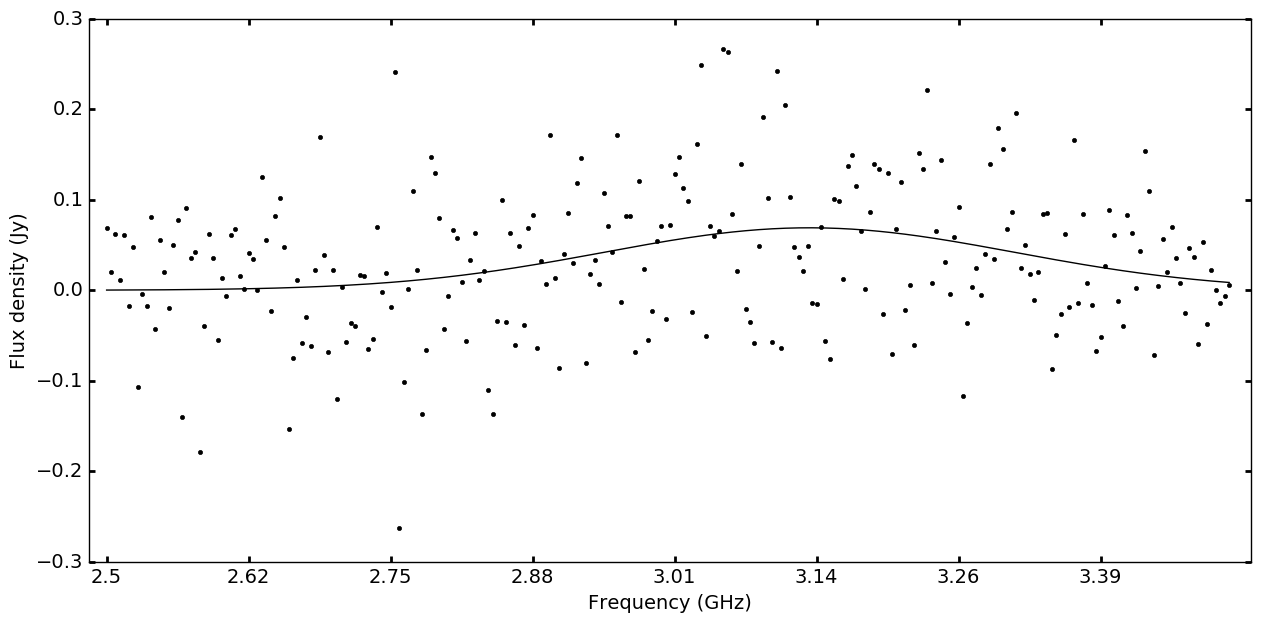
\includegraphics[width=0.33\columnwidth]{spec_57638.png}
  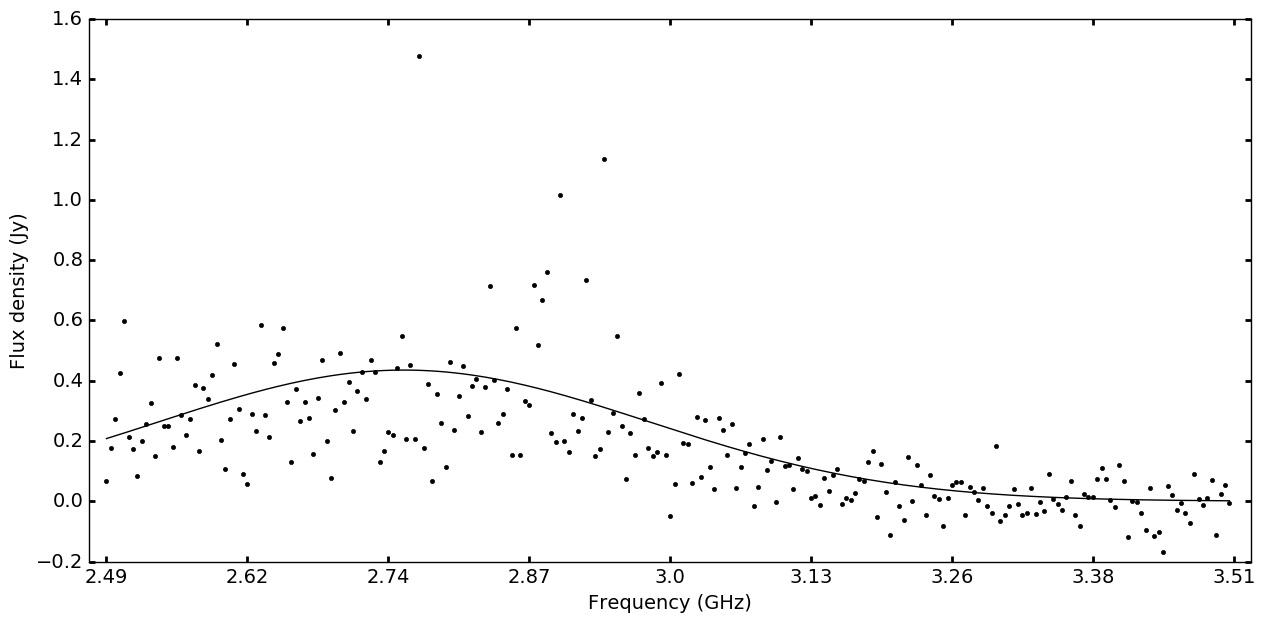
\includegraphics[width=0.33\columnwidth]{spec_57643.png}
  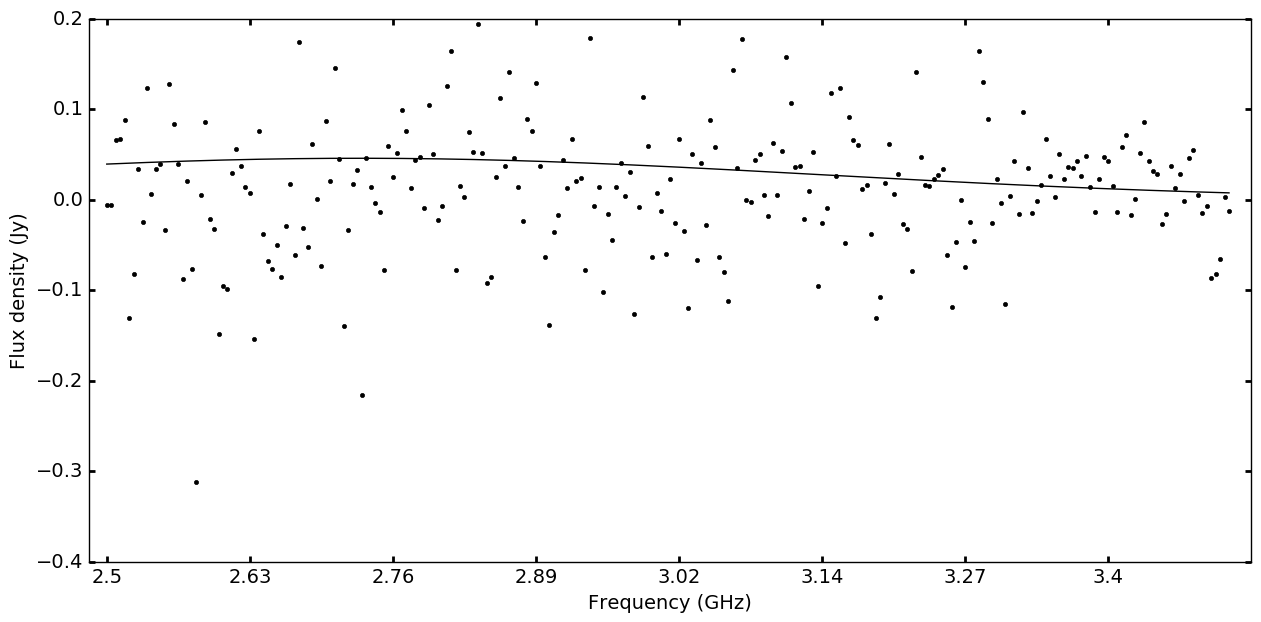
\includegraphics[width=0.33\columnwidth]{spec_57645.png}
 \end{minipage}

 \begin{minipage}{2\columnwidth}
  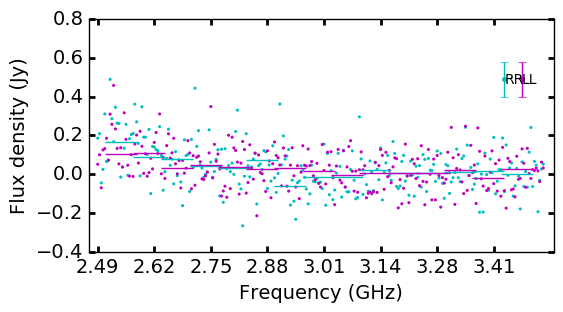
\includegraphics[width=0.33\columnwidth]{spec_57646.png}
  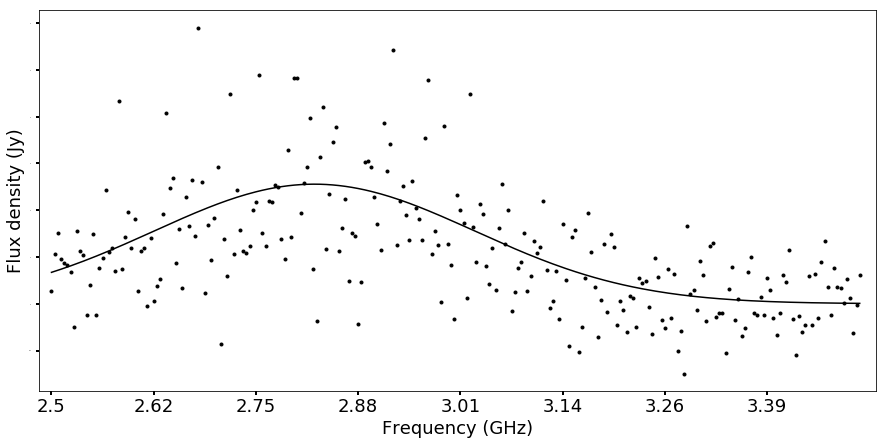
\includegraphics[width=0.33\columnwidth]{spec_57648.png}
  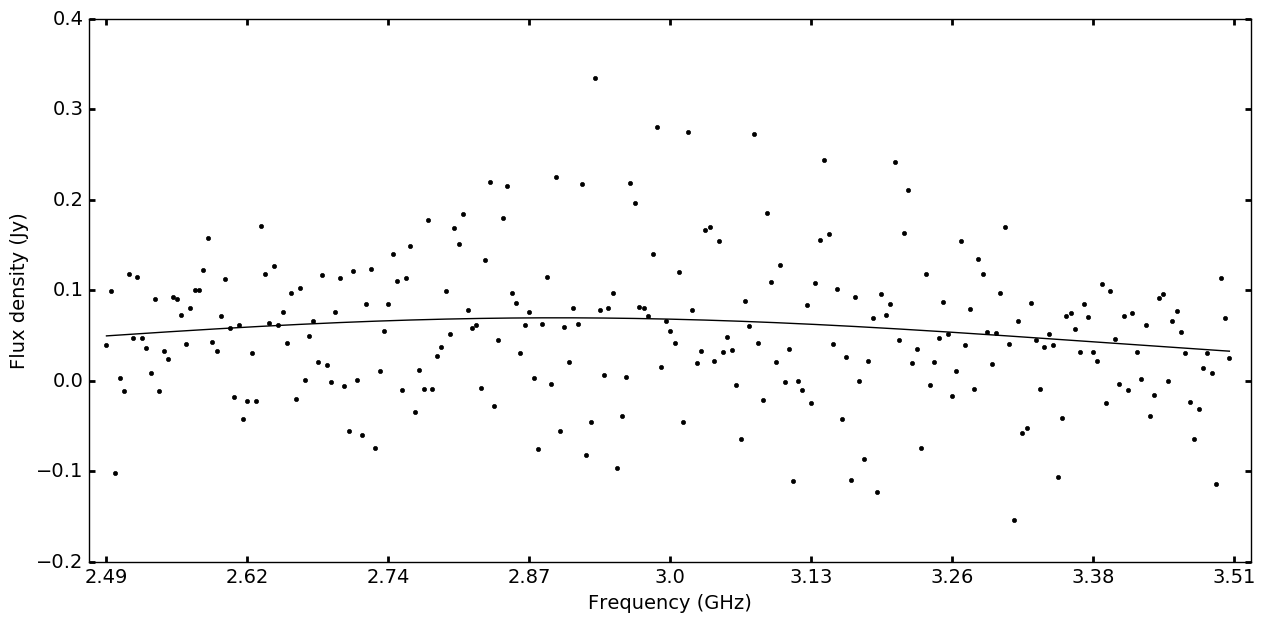
\includegraphics[width=0.33\columnwidth]{spec_57649.png}
 \end{minipage}
\caption{Spectra and best-fit model for nine bursts seen by the VLA from 2.5 to 3.5~GHz. Starting at the top left (moving right and then down), they correspond to bursts on MJDs 57623, 57633.68, 57633.70, 57638, 57643, 57645, 57646, 57648, and 57649. The solid line is a best-fit Gaussian model found through probabilistic modeling. Note that bursts are detected in 5~ms images generated from dedispersed visibilities.
\label{fig:spec}}
\end{center}
\end{figure*}

\subsubsection{Dispersion}
The initial VLA detections were made by searching a DM grid that allowed inter-DM sensitivity losses up to roughly 10\% \citep[$\Delta DM=10\ \rm{pc}\ \rm{cm}^{-3}$][]{2003ApJ...596.1142C}. In optimizing detection significance over a fine DM grid, we find optimal DM values range from 552 to 572 pc cm$^{-3}$. However, the uncertainty in the peak DM measurement is defined by the signal-to-noise of the burst and how this changes with DM.

Given that the apparent DM can potentially change due to intrinsic or extrinsic effects, we developed a more sophisticated system for modeling dispersion. We created a generative model to sample the likelihood distribution as a function of DM \citep{2010arXiv1008.4686H}. We use the Gaussian shape (see \S \ref{sec:spec}) along the spectral axis and apply a frequency-dependent delay for a given dispersion model. The likelihood is directly sampled by calculating the product of probabilities on a per-pixel basis of the 2-dimensional dynamic spectrum. Uncertainties in each pixel are drawn from a uniform Gaussian error distribution that is estimated from the data.

**Does DM correlate with other spectral/flux properties?**

Figure \ref{fig:dmmodel} compares the 95\% confidence intervals on the DM for all nine VLA bursts to the range of DM previous observed \citep{2014ApJ...790..101S,2016arXiv160308880S}. The DM confidence intervals are not consistent with each other or a single DM. This suggests that there are apparent DM changes between bursts, either due to intrinsic burst structure or actual changes to the DM column density. Elsewhere, we present high-resolution dynamic spectra at 1.4~GHz that show how intrinsic spectral structure can bias the apparent DM of individual bursts \citep{WEIRD}. The FRB emission process has not yet been defined, so it is not clear how the intrinsic structure can bias DM as a function of frequency.

\begin{figure}[htb]
\begin{center}
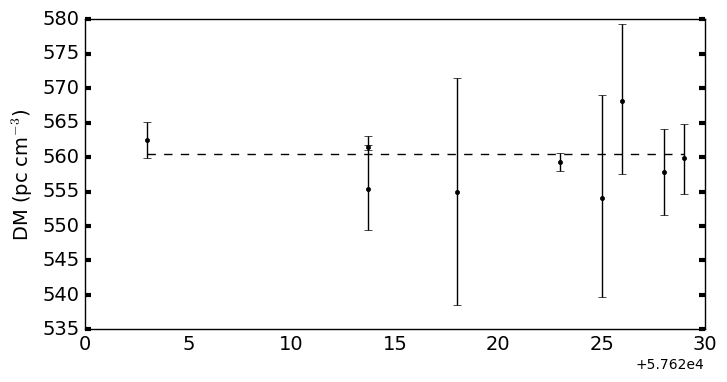
\includegraphics[width=0.9\columnwidth]{dmmodel}
\caption{DM as a function of time for nine 3~GHz bursts detected by the VLA. The 95\% confidence interval on DM is shown with a bar and the dahsed line shows the best-fit DM$=560.5$\ pc cm$^{-3}$ inferred for Arecibo observations at 1.4~GHz (CITE: WEIRD).
\label{fig:dmmodel}}
\end{center}
\end{figure}

% TODO: Non-lambda$^{2}$ dispersion...


\subsubsection{Spectral Autocorrelation}
\label{sec:auto}
Autocorrelation of the burst signal (both temporal and spectral) can be used to infer both intrinsic properties and modulation due to scintillation \citep{CORDES}. Figure \ref{fig:acf} shows the spectral autocorrellation for the strongest burst (MJD 57633.68). The is no strong excess correlation near the channel resolution, which limits the correlation width to less than roughly 4~MHz. This is broadly consistent with expectations of Galactic diffractive scintillation bandwidth \citep[3--9~MHz near 3~GHz][]{2002astro.ph..7156C}.

%**Does channel-scale structure only appear around 3~GHz?**

\begin{figure}[htb]
\begin{center}
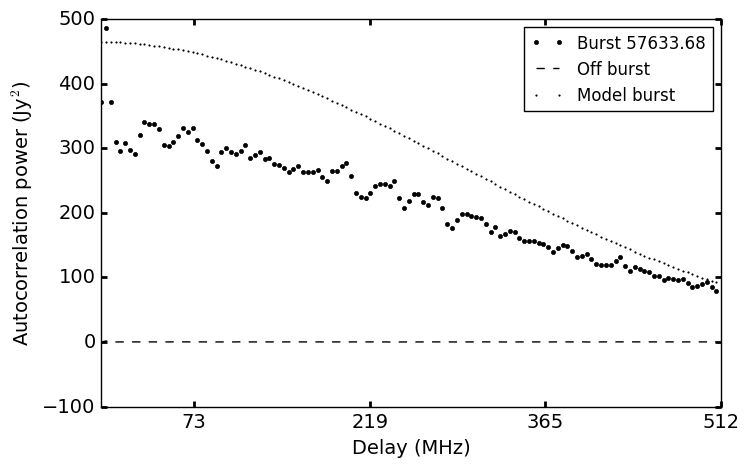
\includegraphics[width=0.9\columnwidth]{acf_57633_scan7}
\caption{The spectral autocorrelation as a function of frequency for the burst from \frb\ at MJD 57633.68. The largest black dots show the autocorrelation for the data, smaller dots show the autocorrelation for the best Gaussian model, and dashed line shows the autocorrelation of an off-burst spectrum.
\label{fig:acf}}
\end{center}
\end{figure}

\subsubsection{Circular Polarization}
The VLA S-band recievers measure circular polarization, although for observing efficiency we choose not to include polarization calibration procedures. Constraints on circular polarization are possible since the gain calibrator is a well-known polarization calibrator with little Stokes V flux. In that case, the apparent circular polarization fraction is $(RR-LL)/(RR+LL)$, which for the most significant bursts is at most 3\%. \frb\ was located 2.3\arcmin away from pointing center, where systematic effects have been measured as large as 3\% (Perley et al 2016, VLA memo). Given that systematic effects dominate the apparent circular polarization, we conclude that the true fractional circular polarization is less than 3\%.

\subsection{Temporal Statistics}
\label{sec:temp}
Geoff comments:
-- need to clarify that burst rate change is significant
-- not clear how significant nondetections are, since observational details not obvious yet

Burst detections were made very inhomogenously through the 2016 observing campaign and total 63 hours. In the early-2016 campaign, we observed for 30 hours at S-band and no bursts were detected. In the late-2016 observing campaign, nine bursts were detected in the last 27 hours of S-band observing. Overall, the data quality is uniform and high, so the inhomogeneous burst distribution shows that the burst detection probability was not stationary. Assuming that the burst detection probability follows a Poisson distribution, the nondetection in the first half of S-band limits the FRB rate to $\rm{R}<0.1$\ hour$^{-1}$\ (95\% confidence limit). The mean detection rate for S-band observing during the late-2016 campaign was $\rm{R}=0.33\pm0.1$\ hour$^{-1}$.

There is weak evidence that the \frb\ burst rate decreased through the S-band observing in the late-2016 campaign. We modeled the event detection probability as a Poisson probability function, $P_i(\lambda)$, with rate parameter that evolves linearly in time relative to the first VLA burst $\lambda = a + b (\rm{MJD}_i - 57623)$. By directly sampling the joint probability distribution, $\prod_{i} P_i$, we can exclude a constant rate with $\sim$85\% confidence. This weak constraint is consistent with the broader trend of a changing rate seen on month timescales by Arecibo.

%\begin{figure}[htb]
%\begin{center}
%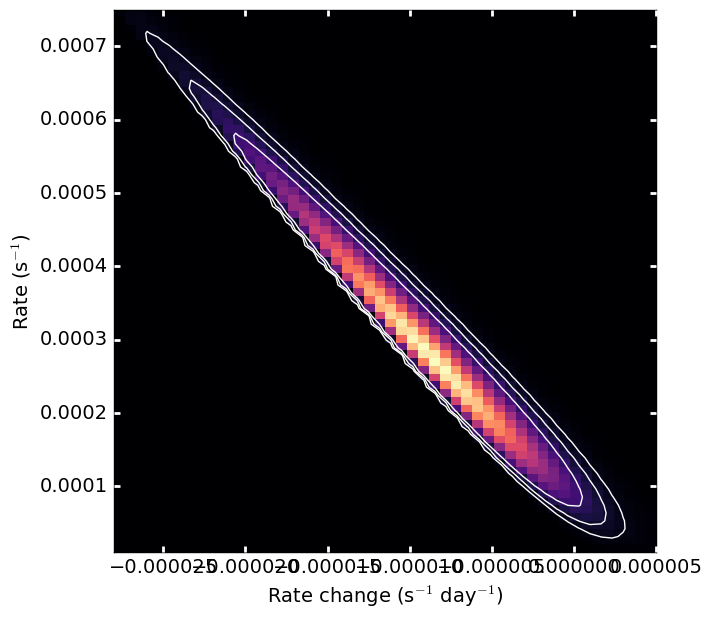
\includegraphics[width=0.9\columnwidth]{event_rate_contours}
%\caption{Color scale and contours show the relative probability for a time-evolving Poisson detection probability for \frb. Contours show the 50, 90, and 95\% confidence contours on the rate $a$\ (bursts s$^{-1}$) and rate change $b$\ (bursts s$^{-1}$ day$^{-1}$) during the August--September 2016 campaign in which bursts were detected.
%\label{fig:rate}}
%\end{center}
%\end{figure}

During the late-2016 observing campaign, the typical observation lasted about two hours and was sampled with a 5~ms cadence. We used the Lomb-Scargle periodogram \citep{1982ApJ...263..835S} to search for periodic structure over a wide range of timescales. The time series is calculated by binning the burst detection rate per 100~ms \citep[always either 0 or 1, see also][]{2011MNRAS.417.1871P}. 
The spectral power calculated for periods between 0.8 and 80 s shows no power in excess of the typical 95\% confidence bound estimated from shuffled data. We verified that simulating nine bursts drawn from a simple rotational model would produce excess power using this approach. However, it is difficult to put strong constraints on more complex rotational models \citep[e.g., with wide pulse phase windows or glitches;][]{2007ApJ...663..497C, 2013Natur.497..591A}

\subsection{Energy and Brightness Distribution}
\label{sec:disn}
Knowing the burst distance, we calculate their total energy by integrating flux in time and frequency (Table \ref{tab:spec}). Some VLA burst spectra seem to be contained by the 2.5 to 3.5~GHz band and most of them seem to have Gaussian envelopes that are well modeled by the emission within the 2.5 to 3.5~GHz band. Assuming that the Gaussian shape defines the emission window, the mean S-band flux density can be converted to a total energy with no further assumptions about their spectral properties. We proceed under this assumption here and discuss caveats later.

The \frb\ burst energy distribution (Figure \ref{fig:ed}) is relatively flat, as seen in the range of significance of the nine bursts (12 to 179$\sigma$). We modeled the differential energy distribution, $dN/d\log{E}$, as a Poisson probability distribution with a rate function $\lambda\proptoE^{\alpha}$. Using a maximum likelihood technique, we estimate the best powerlaw index of $\alpha=-0.6^{+0.4}_{-0.6}$. This is equivalent to a differential energy distribution, $dN/dE \propto E^{-1.6}$. Note that all VLA bursts are much brighter than the sensitivity limit ($8\sigma$) and data quality are relatively uniform and good, so the distribution is not affected by a completeness limit.

\begin{figure}[htb]
\begin{center}
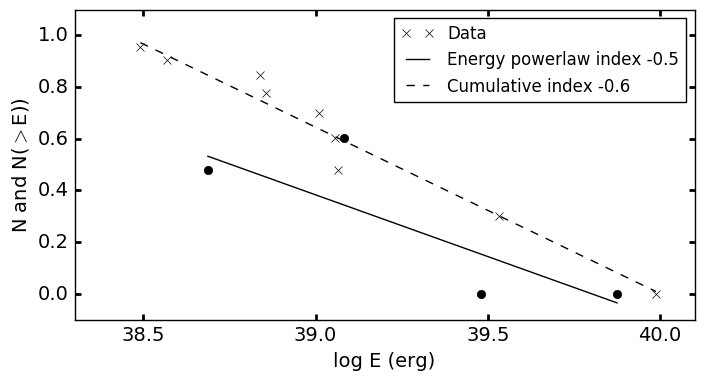
\includegraphics[width=0.9\columnwidth]{energy_disn}
\caption{Dots and solid line show the  \frb\ burst energy cumulative distribution. The dashed line shows the best fit from a maximum likelihood analysis using the powerlaw model $dN/d\log{E} \propto E^{\alpha}$. The 95\% bounds on the best-fit powerlaw index is $\alpha=-1.6^{+0.4}_{-0.6}$. \label{fig:ed}}
\end{center}
\end{figure}

\section{discussion}

\subsection{Emission Physics and Burst Energetics}
The refined analysis shows that \frb\ has even higher isotropic energies than previously reported, reaching energies $E_{\rm{max}}\approx10^{40}$\ erg. We now know that \frb\ is detectable with the VLA out to $z=0.7$\ and much farther with Arecibo. \frb\ has isotropic energies orders of magnitude higher than the strongest Crab pulsar pulses ($\sim10^{35}$~erg) and comparable brightness temperatures \citep[$T_b^{\rm{Crab}}\sim10^{41}$~K versus $T_b^{\rm{FRB 121102}}\sim10^{38}$~K;][]{2003Natur.422..141H,2014PhRvD..89j3009K}. While this emission is coherent and strongly beamed \citep{2016Natur.531..202S, WEIRD}, the energy scale is still larger than any Galactic class of fast radio transient and requires either a new process or dramatic scaling of known emission processes \citep{2016MNRAS.462..941L, 2016MNRAS.457..232C}.

Propagation effects (e.g., scintillation, scattering) can also modify the radio signal in a variety of ways and the duration of the emission in the source frame is not known \citep{2016arXiv160505890C}. \citet{CORDES} describe a model where plasma lensing near the source of an FRB can magnify radio emission by orders of mangitude. That model argues that the simultaneous appearance of a burst from 1.2 to 3.5~GHz requires a lens with the focal frequency be $\gtrsim 3.5$~GHz. This gives a constraint on the combination 
$$\frac{\rm DM_0}{a_{\rm AU}^2} \frac{d_{sl}d_{lo}/d_{so}}{1\, \rm kpc} \gtrsim (3.5 / 39.1)^2$$
where $DM_0$, $a$, and $d_*$\ are the electron column density of the lens, size of the lens, and lensing distances, respectively. A lens placed at $d_{sl}\approx1$~kpc is consistent with typical properties of the interstellar medium. Lenses that are influenced by the source would be much nearer to the source $d_{\sl} \ll 1$~kpc, requiring large values of $\frac{\rm DM_0}{a_{\rm AU}^2}$.

\subsection{FRB Flux Distribution}
The Lorimer burst was surprising for its unusually large flux with a lack of lower-significance detections. As more FRBs have been detected, it has become clear that the FRB population has a relatively flat flux distribution \citep[cumulative flux distribution index $-0.5<\alpha<-1$;][]{2016ApJ...830...75V, 2016arXiv160206099L, 2016arXiv161100458L}. This fact was recently demonstrated by yet another detection of an extremely bright FRB \citep{2016arXiv161105758R}.

Assuming that the \frb\ energy distribution is typical of FRBs, we can use it to simulate FRB populations and compare their flux distributions to the observed distribution. First, we assume an FRB population that is uniformly distributed in space from redshifts $z1$\ to $z2$. For each FRB source, we sample one FRB burst luminosity from a powerlaw distribution and calculate its flux.
%(uniform for energies from $10^{38}$\ to $10^{40}$; \S \ref{sec:disn} 
We sample 100 such populations and measure 95\% bounds on the distribution of cumulative flux distribution index.
We can show that the flux distribution powerlaw is --1.5 for a standard candle-like luminosity distribution at low redshift. For distributions out to $z2>1$, the distribution flattens slightly ($sim0.3$ in the index) due to cosmological space distortions.
For a large ($N\sim2000$) population of such bursts, we select the brightest $M\sim20$\ to represent the flux-limited FRB sample of known FRBs...
The tail of this distribution selects for extrema, such cut-offs in the intrinsic distribution or propagation effects \citep{2015MNRAS.451.3278M, CORDES}. 
We then fit the flux distribution of those $M$\ events with a powerlaw.

These simulations confirm previous work that shows that...
The cumulative flux distribution follows a Euclidean distribution \citep[index $=-1.5$;][]{2016MNRAS.462..941L} when...
Flatness has been observed...
This requires...


It is not yet clear whether \frb\ can be treated as a representative of the broader FRB population. \citet{2016Natur.531..202S} describes burst spectral structure that is intrinsic, or at least dominated by propagation effects close to the emitting region. On the other hand, \citep{CORDES} have identified a variety of propagation effects in our own Galaxy that can plausibly modify the observed brightness distribution.


**caveats of S-band assumption**

\subsection{Repetition}
The burst rate analysis presented in \S \ref{sec:temp} shows that the detection probability of \frb\ is not stationary. As mentioned above, this could be caused by intrinsic events (e.g., magnetar outburst) or propagation effects. While a detailed analysis of temporal correlation will require more bursts and/or more sophistication, it is clear that \frb\ has significant correlation on short timescales \citep[sometimes called a ``red spectrum'';][]{2016MNRAS.458L..89C}. Another way of stating this is that the detection of a burst improves odds of finding more bursts in near-future observations. 

If this statistical property describes other FRBs, it weakens previous constraints on repetition \citep{2015MNRAS.454..457P,2015ApJ...807...16L}. It is possible that other FRBs have repeating bursts, although calculating a limit requires knowing the temporal correlation function that defines the repetition.  Repetition also implies that there are fewer phyiscal sources of FRBs than implied by the burst detection rate.

FRBs like SGRs? 2016ApJ...826..226K

\subsection{FRB Rate}
% cut from gemini paper. TODO: incorporate referee comments on rate scale. Sarah?
{\color{red} Sarah: can you update this as a per-SFR rate?}
Assuming that \frb\ is from the same population as the other FRBs, the measurement of a distance for the host of \frb\ allows us to re-evaluate the cosmic volume and event rate per galaxy for the FRB population. The estimated projected FRB rate $R_p$\ understates the true rate by a beaming fraction $\Omega_b$\ \citep[$\sim$10\%;][]{1998MNRAS.298..625T}. For a comoving volume $V(z)$\ and galaxy number density $\Phi(M)$, the rate per galaxy is $R_{FRB} = R_p /(\Omega_b \Phi(M)V (z))$. 

The first such rate estimate was made by \citet{2013Sci...341...53T}, who used the measured DM to estimate a characteristic distance for their sample of 4 FRBs. They assumed that all of the extragalactic component of the DM was caused by the IGM and scaled as $DM\approx z\times1200 \rm{pc}\ \rm{cm}^{-3}$\ \citep{2003ApJ...598L..79I,2004MNRAS.348..999I}. They also calculated the number of galaxies by assuming a characteristic $L_*$\ galaxy \citep[corresponding to stellar mass $M_* \approx 1011 M$;][]{2012MNRAS.421..621B}.

**add error bar?**
Our calculation differs in that we have better estimates of all three parameters. First, the projected FRB rate is now believed to be closer to $2\times10^3\ \rm{sky}^{-1} \rm{day}^{-1}$\ at high Galactic latitudes and flux densities brighter than 1 Jy ms \citep{2016arXiv161100458L,2016MNRAS.460L..30C, 2016MNRAS.455.2207R}. \frb\ is associated with a relatively small galaxy ($5\times10^7$\ Msun), which are roughly a factor of 100 more abundant \citep[$\Phi(M) \approx 10^{-2} \rm{Mpc}^{-3}$;][]{2007ApJ...665..265F}. Finally, the measured distance for FRB 121102 suggests that the extragalactic DM has comparable contributions from the IGM and host galaxy.

This reduces the characteristic distance by a factor of two and the volume by an order of magnitude. Considering these factors, we assume a characteristic redshift of the population that is twice that of \frb\ to estimate $R_{FRB} \approx 10^{-4} (0.1/\Omega_b) \rm{galaxy}^{-1} \rm{year}^{-1}$, which is two orders of magnitude lower than previously estimated \citep[assuming isotropic radiation;]{2013Sci...341...53T}.

There are significant caveats to the comparison of this rate to the rates of other classes of transient. This isotropic FRB rate assumes a projected FRB rate at a single (observationally defined) flux limit and that no bursts repeat. Using this calculation with data from more sensitive telescopes, we might infer a higher rate. However, if we assume that \frb\ is representative of the overall FRB population, then more sensitive observations would be more likely to find repeating FRBs that would effectively depress the estimate of the underlying isotropic rate per source. In this model, these two effects partially cancel, although without a physical model it is difficult to say how well.

\subsection{Observing Strategies}
As discussed above, \citet{2016MNRAS.458L..89C} note that the FRB repetition implies that the number of FRB-generating sources is smaller than implied by the number of bursts. In some scenarios, this means that there are areas on the sky that may contain no FRBs. Wide, shallow surveys are the preferred strategy for blind detection of FRBs. However, future efforts to localize FRBs are still most likely to succeed by targeting known FRBs to catch repetitions, assuming that all FRBs repeat. Finally, we note that the average spectral coverage of bursts from \frb\ are relatively narrow ($<1$~GHz) and the coverage changes dramatically between bursts. Thus, the odds of detecting a burst will improve linearly with bandwidth for bandwidths wider than this characteristic scale.

%\subsection{Naming Convention}
%The consistency of \frb\ properties (e.g., energy distribution) with the overall population suggests other FRBs likely repeat. If so, the current naming convention for FRBs (analogous to cataclysmic supernovae), will likely become uninformative, especially as large FRB survey projects come online \citep{2014SPIE.9145E..22B}. If all FRBs repeat, then a more useful convention would be based on coordinates. However, there are already two FRBs that have consistent celestial positions and different DMs. Therefore, we suggest an FRB naming convention as Jhhmm+ddDMmmmm.

\section{Conclusions}
Prior to being established as a cosmological source, the low Galactic latitude of \frb\ made it a somewhat compromised member of the FRB class. With its cosmological distance firmly established, \frb\ now serves as a new kind of standard by which FRBs are defined. That fact, combined with an abundance of data collected during its high activity state, allows us to think more generally about the physics of broader FRB population.

We presented the first multi-telescope detection (Arecibo and VLA) of an FRB. By detecting this burst from 1.2 to 4.5~GHz, we have demonstrated that some bursts have broad spectral structure. However, three other VLA bursts are undetected by Arecibo. That, combined with the measurement of spectra within the VLA band, suggest that the typical burst has a characteristic Gaussian spectral shape with width $\sim500$\ MHz.

**Flux/lum distribution**

Analysis of the VLA burst times shows that the burst rate is highly variable. This shows that past constraints on FRB repetition are weaker than previously inferred. The combination of relatively narrow spectral structure, flat energy and flux distributions, and variable burst rate suggests that repeated observations, wide bandwidth, and large instantaneous field of view all improve the chance of detection. 

New, arcsecond-scale localizations will continue to be highly informative, given that FRB hosts may be faint and can confuse the inference of a properties of the intergalactic medium \citep{2014ApJ...783L..35D}. \frb\ was localized within hours by a prototype version of \rf, but an expanded \rf\ system is now under construction. This platform will search a TB/hour data stream in real time in parallel with ongoing VLA observations, potentially detecting and localizing multiple FRBs per year. {\color{red} Sarah: any refinement to this statement?} VLASS+\rf?

\bibliographystyle{apj}

\section*{Acknowledgements}
% observatories
The National Radio Astronomy Observatory is a facility of the National Science Foundation operated under cooperative agreement by Associated Universities, Inc..
% systems
This research made use of Astropy, a community-developed core Python package for Astronomy (Astropy Collaboration, 2013).
%individuals
CJL is supported by the University of California Office of the President under Lab Fees Research Program Award 237863 and NSF award **number**.
MAM is supported by NSF award \#1458952. 
KPM's research is supported by the Oxford Centre for Astrophysical Surveys which is funded through the Hintze Family Charitable Foundation. AS gratefully acknowledges support from the European Research Council under grant ERC-2012- StG-307215 LODESTONE. The AMI-LA telescope gratefully acknowledges support from the European Research Council under grant ERC-2012- StG-307215 LODESTONE, the UK Science and Technology Facilities Council (STFC) and the University of Cambridge.


\bibliography{fasttrants.bib}

%\begin{figure}[htb]
%\begin{center}
%\includegraphics[width=0.9\columnwidth]{}
%\caption{
%\label{fig:name}}
%\end{center}
%\end{figure}

%\begin{table}
%\caption{Caption}
%\footnotesize
%\centering
%\begin{tabular}{l|cc|cc|c}
%\hline
%Field       & RA          & Dec   & Lon. & Lat.     & Time \\
%            & \multicolumn{2}{|c|}{(J2000)}  & \multicolumn{2}{|c|}{(Galactic; deg)} & (hrs) \\ \hline
%RA02        & 2:27:53  &  +9:13:24 & 159.0 & --46.8    & 26.25 \\
%PSR J2248-0101 & 22:48:27 & --1:1:48 & 69.3 & --50.6 & 6.5 \\ \hline
%\end{tabular}
%\label{fields}
%\end{table} 

\end{document}

